\chapter{Umsetzung}


Nachdem in dem vorhergegangenen Kapitel der Entwurf für die Erstellung des Adobe PDF Formulars erarbeitet wurde, wird in diesem Kapitel die Umsetzung an Hand dieses Entwurfs erläutert.
Hierfür wird zunächst die Migration der Schnittstelle beschrieben, gefolgt von der Erstellung des Formulars. 
 

\section{Schnittstelle}

Für die Migration der Schnittstelle wird in der Transaktion "`SMARTFORMS"' das relevante Formular ausgewählt. Anschließend wird über den Menüpunkt "`Hilfsmittel"' die Migration zu einer Interactive Form ausgewählt. Daraufhin wird als Zielformular der gewünschte Name der Schnittstelle sowie des Formulars eingetragen. Hiernach können Einstellungen für die Migration vorgenommen werden. In Abbildung \ref{mig-einst}
 sind die Standardeinstellungen dargestellt, welche für die Migration der \ac{LLE} verwendet werden.
 
 \begin{figure}[ht]
 	\centering
 	\makebox[\textwidth][c]{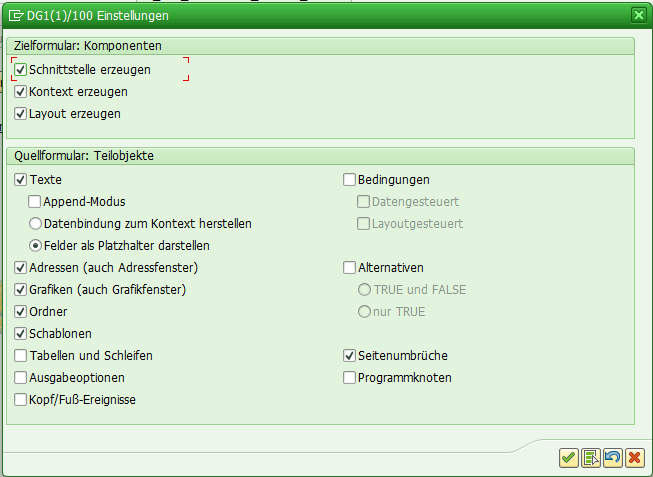
\includegraphics[width=9 cm]{img/mig-einst.png}}%		
 	\caption{Einstellungen der automatischen Migration von Smart Forms zu Interactive Forms}
 	\label{mig-einst}
 \end{figure}

Nachdem diese Einstellungen bestätigt wurden ist die Migration abgeschlossen. Abschließend wird noch ein Protokoll angezeigt, welches bereits erkannte Fehler\footnote{Siehe Kapitel \ref{Migration}} des neuen Formulars auflistet. Nachdem die Migration abgeschlossen ist, wird die Schnittstelle auf Fehler überprüft und anschließend aktiviert. 

\FloatBarrier
\section{Formular}
\subsection{Allgemein}

Das Formular, welches im Laufe der automatischen Migration erstellt wurde, wird nicht verwendet. Stattdessen wird nach dem Erstellen der Schnittstelle ein Formular in der Transaktion SFP angelegt. Im Anlageprozess muss unter anderem die zugehörige Schnittstelle angegeben werden. Nachdem das Formular angelegt wurde kann mit der weiteren Erstellung des neuen Dokuments begonnen werden.

Für diverse Texte des Formulars müssen Textbausteine angelegt werden. Diese werden in der Transaktion "`SMARTFORMS"' erstellt. Der genaue Prozess der Textbausteinerstellung ist jedoch sehr komplex und wird somit nur wie folgt zusammengefasst: Ein Textbaustein wird erstellt und mit dem relevanten Text gefüllt. Parallel wird dem Textbaustein ein "`Stil"' zugewiesen. Dieser Stil gibt bestimmte Formatierungsmöglichkeiten vor, mit deren Hilfe kann der Text wie gewünscht formatiert werden.

\subsection{Anschreiben der \acs{ABB}}

Für das Anschreiben werden zunächst im Kontextbereich die benötigten Daten hinzugefügt. Relevant für das Anschreiben sind die diversen Adressdaten\footnote{Siehe Kapitel \ref{ist:adr}} sowie die Angaben bezüglich des Gültigkeitszeitraums der \ac{LLE}. Für die Absenderadresse wird ein Adresselement angelegt. Dieses Element wird mit der Adressnummer der Absendergesellschaft gefüllt. Des Weiteren werden die Grafikelemente für die Logos angelegt und mit den Namen der zugehörigen "`GRAPHICS"' Objekte versehen. Abschließend werden noch die Textbausteine für die Fußzeilen im Kontextbereich in Form eines Textelements eingebunden. Hierbei werden die Grafikelemente, das Adresselement, sowie die Fußzeilen mit Bedingungen versehen, welche die \ac{AH} Nummer abprüft. Die Namen der verschiedenen Elementen sind dabei so gewählt, dass erkennbar ist, welche Funktion dieses Element besitzt. Beispielsweise heißt das Grafikelement des \ac{BJE} Logos "'LOGO\_BJE"'. 

Nachdem der Kontextbereich für das Anschreiben fertiggestellt ist wird das Layout bearbeitet. Zunächst wird eine Masterseite und eine Inhaltsseite für das Anschreiben erstellt. Mit Hilfe der Objekt-Palette\footnote{Siehe Kapitel \ref{ch:Aufbau}} wird die Masterseite von der Nummerierung ausgeschlossen. Auf der Inhaltsseite werden zunächst die Grafikelemente der Logos hinzugefügt. Die Position und Größe wird hierbei aus dem Smart Forms-Formular übernommen. Anschließend werden die Inhaltsbereiche für die Adressköpfe erstellt. Die Empfängeradresse richtet sich hierbei an die Position des Fensters in einem Briefumschlag. Über der Empfängeradresse wird die Rücksendeadresse eingesetzt. Beide Adressfelder werden mit Fließtextfeldern gefüllt. In Abbildung \ref{if:adr} sind die, durch geschweifte Klammern gekennzeichnete, Fließtextfelder abgebildet.

 \begin{figure}[ht]
	\centering
	\makebox[\textwidth][c]{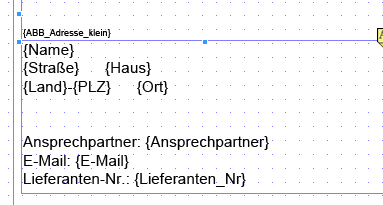
\includegraphics[width=9 cm]{img/ist-adr.png}}%		
	\caption{Fließtextfelder im Adresskopf}
	\label{if:adr}
\end{figure}

Der Adresskopf des Absenders der \ac{LLE} wird in einer ähnlichen Weise, nur auf der rechten Seite des Dokumentes eingefügt. Die Position des Feldes richtet sich hierbei nach dem Smart Forms-Formular\footnote{Siehe Kapitel \ref{ist:adr}}. Über der Absenderadresse wird das automatische Adressfeld für die Absender Gesellschaft eingesetzt. Das Feld muss lediglich ausgerichtet beziehungsweise positioniert werden.  Eingefügt werden, kann das Feld per Drag\&Drop aus der Datenansicht heraus.

Anschließend an die Adressköpfe wird der Inhaltsbereich für den Text des Anschreibens erstellt. Der Text wird hierfür direkt aus dem alten Formular kopiert und eingefügt. Die Formatierung wird angepasst bezüglich fettgedruckten Inhalten und Absätzen. Die dynamischen Inhalte des Textes werden in Fließtextfelder umgewandelt und über die Objekt-Palette an die zugehörigen Daten gebunden.

Abschließend werden die beiden Fußzeilen am unteren Ende des Dokumentes eingefügt. Die Dimensionen der Textfelder wird dem Smart Form-Formular entnommen. Wie auch bei dem Adressfeld können diese Elemente ebenfalls per Drag\&Drop aus der Datenansicht in das Formular eingesetzt werden. Positioniert werden die Textelemente so, dass sie sich unter dem Inhaltsbereich des Anschreibens befinden.


\subsection{Anschreiben der \acs{LLE}}
	
Analog zur ersten Seite wird auch für das Anschreiben der \ac{LLE} eine Masterseite und eine Inhaltsseite erstellt. Entgegengesetzt zur vorhergegangenen Seite wird dieses Anschreiben jedoch in die Nummerierung der Seiten mit einbezogen. Anschließend wird auf der Masterseite eine Seitenangabe hinzugefügt. Eine Vorlage für ein Standard "`Seite X von XX"' Format steht in der Bibliothek des \ac{ALCD} zur Verfügung. Dieses Element passt sich dynamisch an die aktuelle Seite an und zählt auch nur die Seiten mit, welche für die Nummerierung mit einbezogen werden. Dieses Feld wird auf der Seite ganz unten in der Mitte platziert.
Die restliche Seite wird mit einem Inhaltsbereich ausgefüllt für den Text des Anschreibens. Dieser Text wird zunächst aus dem alten Formular kopiert und im neuen Formular, mit der gleichen Formatierung, eingefügt. Die dynamischen Inhalte werden erneut mit Fließtextfeldern eingesetzt. Abschließend wird für die erste Seite des Formulars noch eingestellt, dass die Folgeseite das \ac{LLE} Anschreiben ist. 
	
	
	\FloatBarrier
\subsection{Materialliste}

Für die Seiten der Materialliste wird erneut eine Masterseite und eine Inhaltsseite erstellt. Diese Seiten werden in die Nummerierung mit einbezogen und werden zusätzlich im Querformat dargestellt. Nachdem die Seite erstellt wurde, wird wiederum die Seitenangabe am Ende der Seite eingefügt. Des Weiteren wird ein Inhaltsbereich für die Kopfdaten der Materialliste erstellt. Die Position sowie die Inhalte dieses Bereiches werden aus dem Smart Form Formular übernommen. Die dynamischen Inhalte werden wiederum mit Fließtextfeldern eingefügt. 

Für die Tabelle wird zunächst der Kontextbereich des Formulars erweitert. Es wird ein Knotenpunkt in Form eines Ordners erstellt, welcher die Elemente der Tabelle beinhalten soll. In diesem Ordner wird anschließend eine Schleife angelegt. Im Fall der \ac{LLE} soll jeder Eintrag der Materialliste im Layout angezeigt werden. Demnach wird in der angelegten Schleife die Materialliste angegeben. Innerhalb der Schleife wird dann eine Zeile dieser Tabelle als Struktur eingetragen. Diese Zeile wird beim erstellen des Formulars mit jedem Eintrag der Materialliste gefüllt. Zusätzlich wird eine Programmknoten in die Schleife eingefügt. Diese Programmlogik wird benötigt um Teile der Materialliste für die Darstellung auf dem Formular aufzubereiten.

Nachdem der Kontext Bereich angepasst wurde, wird anschließend die Tabelle im Layout eingebaut. Zunächst wird mit Hilfe des Tabellen-Assistenten des \ac{ALCD} eine Tabelle mit 7 Spalten erstellt. Diese Tabelle wird in einem Teilformular umschlossen. Anschließend wird in der Objekt Palette der Tabelle der Seitenumbruch freigegeben. Des Weiteren wird in der Palette der Kopfzeile eingestellt, dass der Kopf auf jeder umgebrochenen neuen Seite erneut angezeigt werden soll. Um einen Seitenumbruch in Mitten einer Zeile zu vermeiden, wird für die Zeilen ein Umbruch in der Palette nicht erlaubt. 

Nachdem noch weitere Layout Einstellungen, wie Zeilenhintergründe und Größe, vorgenommen wurden, wird anschließend der Inhalt der Tabelle festgelegt. Wie in Abbildung \ref{figTab} zu sehen ist, werden die Daten der Tabelle ebenfalls mit Fließfeldern abgebildet. Aufgrund der vorher festgelegten Schleife wird somit für jeden Eintrag der Materialliste eine neue Zeile ausgegeben.

\begin{figure}[ht]
	\centering
	\makebox[\textwidth][c]{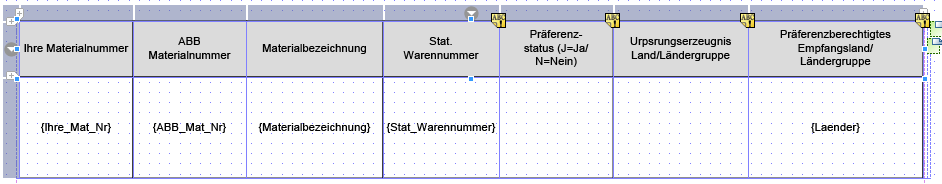
\includegraphics[width=1\textwidth]{img/Tabelle.png}}%		
	\caption{Materialliste mit Fließfeldern}
	\label{figTab}
	
\end{figure}

Um das Layout der Seiten nach einem Umbruch festlegen zu können, wird abschließend in der Objekt-Palette der Seite festgelegt, welche Masterseite für diese Seiten benutzt werden soll. Ansonsten würde die Tabelle auf einer leeren neuen Seite umformatiert weitergeführt werden.

\FloatBarrier
\subsection{Legende}

Die Legende hat strukturell den selben Aufbau wie das Anschreiben der \ac{LLE}, wodurch für beide Seiten die selbe Masterseite verwendet werden kann. Für die Legende wird dementsprechend nur eine Inhaltsseite angelegt, welche der Masterseite des Anschreibens zugeordnet wird. Anschließend wird auf der Inhaltsseite der Textbaustein für die Legende eingefügt. Abschließend wird für die vorhergegangenen Seite eingestellt, dass nach der Tabelle, solange keine weiteren Einträge vorhanden sind, auf die Seite der Legende weitergeführt wird.


\section{Abschluss der Umstellung}

Nach der Fertigstellung des Formulars gilt es, die neue PDF Form im Customizing jeder Gesellschaft zuzuordnen. Nachdem diese Einstellung vorgenommen wurde, kann nun die \ac{LLE} in Form einer PDF ausgegeben werden. Weitere Anpassungen sind nicht nötig.


